\chapter{Gambaran Umum}
\label{chap_overall}

PintarOS merupakan sistem operasi untuk \emph{smart card}. Desain sistem operasi akan mengikuti sebagian dari standard ISO 7816 yang mengatur berbagai aspek mengenai \emph{smart card}.

pintarOS dirancang sebagai sebuah sistem operasi yang generic, yang memiliki tingkat keterbebasan yang tinggi terhadap hardware sehingga tidak terbatas pada arsitektur komputasi tertentu. Meskipun sebagai awal dikembangkan untuk smart card berbasis 8051, pintarOS dirancang agar dapat dengan mudah diimplementasikan pada arsitektur mikroprocessor lainnya ataupun platform tertentu. 

PintarOR dirancang sebagai sistem operasi yang bersifat \emph{platform independent} sehingga tidak terbatas pada platform hardware tertentu saja. Sebagai awal pintarOS akan diimplementasikan pada smart card berbasis mikroprosesor AT90S8515 dan EEPROM 24Cxx atau yang lebih sering disebut \emph{funcard}, namun nantinya akan dapat diimplementasikan (porting) pada berbagai smart card dengan platform hardware lainnya menggunakan desain dan kode sumber yang sama dengan perubahan yang minimum. Sifat platform-independent ini dapat dicapai dengan memisahkan bagian sistem yang bergantung pada platform hardware dalam sebuah modul tersendiri dan yang disebut HAL (Hardware Abstraction Layer), yang menyediakan antarmuka yang sama untuk setiap platform hardware bagi bagian-bagian sistem lainnya.

\subsection{Arsitektur Sistem}
\label{pintaros-arsitektur}

PintarOS dirancang sebagai sistem yang modular, dimana setiap module memiliki fungsi-fungsi yang berbeda. Gambar x menampilkan arsitektur yang digunakan oleh pintarOS, dimana terdiri dari beberapa lapisan. Di bagian paling dasar adalah lapisan Hardware yang menjadi platform dari smart card sendiri, sementara di bagian paling atas adalah lapisan aplikasi. PintarOS berada diantara keduanya, yang memungkinkan aplikasi berjalan diatas platform smart card.

Sebagian dari sistem operasi pintarOS ini diletakkan pada memory ROM/Flash dari smart card : HAL Driver, transmission handler, general command handler, etc. sementara sebagian lainnya diletakkan pada EEPROM. Bagian yang diletakkan pada pada ROM/Flash merupakan kode-kode program dari setiap module-module. Sementara yang diletakkan pada EEPROM merupakan data-data yang akan digunakan oleh pintarOS dalam menjalankan fungsinya seperti Cryptography Key, 

Sebagaimana telah disebutkan, pintarOS dirancang secara modular. Modul-modul utama dari pintarOS ini ditampilkan pada Gambar \ref{fig-arch}. Modul-modul ini dipisahkan menjadi dua bagian, yaitu hardware-dependent dan hardware-independent. bagian hardware-dependent terutama terdiri dari modul-modul hardware abstraction layer (HAL). Modul-Modul ini berfungsi seperti driver yang mengabstraksi hardware pada software sehingga fungsi-fungsi hardware dapat digunakan dengan cara yang sama sebagai sebuah layanan oleh modul lainnya meskipun menggunakan platform hardware yang berbeda.

\begin{figure}[!h]
\centering
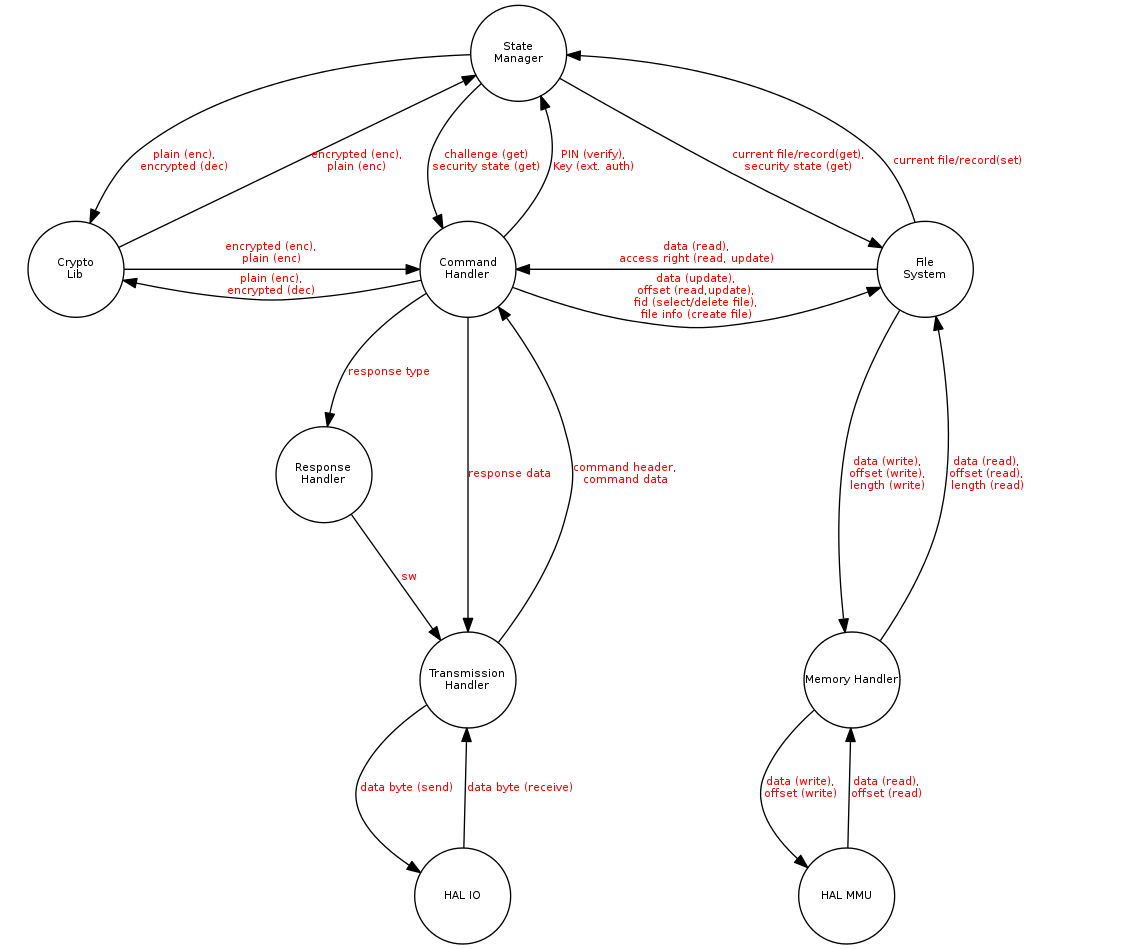
\includegraphics[width=0.75\textwidth]{image/overall/arch.png}
\caption{DFD Keseluruhan Sistem}
\label{fig-arch}
\end{figure}

Berikut adalah penjelasan fungsi dari setiap modul:

\begin{description}
  \item[Hardware Abstraction Layer (HAL)] \hfil \\
berfungsi menyediakan abstraksi dari hardware yang ada dan menyediakan layanan yang sama pada module-module di lapisan yang lebih tinggi meskipun menggunakan platform hardware yang berbeda.
  \item[Transmission Handler]  \hfil \\
bertanggung jawab menangani protokol transmisi yang dipilih untuk berkomunikasi dengan terminal.
  \item[Memory Handler]  \hfil \\
bertanggung jawab menangani pembacaan dan penulisan data secara umum dan generic pada media penyimpanan yang ada
  \item[Command Handler]  \hfil \\
bertanggung jawab menginterpretasikan APDU Commmand dan memanggil command handler yang sesuai,yang kemudian akan melaksanakan instruksi sebagaimana yang diminta oleh command APDU. Setiap instruksi dijalankan menggunakan pendekatan yang sama berdasarkan pada context command APDU. Setiap instruksi yang didukung harus memiliki command handlernya masing-masing.
  \item[Response Manager]  \hfil \\
berfungsi membentuk pesan response APDU (SW1 \and SW2) berdasarkan response type dari command handler.
  \item[File System]  \hfil \\
berfungsi menangani segala hal mengenai file. 
  \item[State Manager]  \hfil \\
berfungsi menyimpan state smart card. Beberapa modul akan menggunakan state ini dalam menjalankan fungsinya, seperti File System membutuhkan informasi mengenai file yang sedang dipilih ketika akan membaca sebuah file.
  \item[Crypto Lib]  \hfil \\
menyediakan layanan kriptografi seperti enkripsi dan dekripsi.

\end{description}

\subsection{File System}
\label{overview}

Bagian ini menjelaskan secara umum mengenai \emph{file system} yang akan digunakan pada \emph{pintarOS}. Sebagaimana dapat dilihat pada rancangan utama, \emph{file system} berfungsi menangani struktur file dan operasi-operasi yang dapat dilakukan terhadap file tersebut. Bagaimana data file tersebut disimpan pada memory fisik tidak menjadi tanggung jawab File System karena akan dilakukan oleh \emph{HAL Memory} dengan  menyediakan layanan untuk penyimpanan dan pengambilan data dari Non-Volatile Memory (NVM) menggunakan pengalamatan yang linier dan kontinyu.

\subsubsection{Struktur File System}
\label{file-system-structure}

Sebagaimana dijelaskan pada dokumen ISO 7816-4, terdapat dua jenis file dasar yang dapat digunakan pada \textsl{smart card} yaitu :
\begin{itemize}
\item Elementary File (EF), dan
\item Dedicated File (DF).
\end{itemize}

\emph{Elementary File} merupakan jenis file yang dapat menyimpan data aktual. Sedangkan \emph{dedicated File} merupakan file khusus yang tidak berfungsi menyimpan data aktual, melainkan memuat daftar sejumlah file lainnya (dapat berupa EF maupun DF). Fungsi DF ini dapat disamakan dengan fungsi \emph{directory} pada komputer PC. Dengan mengelompokkan sejumlah file yang saling berkaitan dalam sebuah DF (sebagai contoh dalam sebuah aplikasi) akan menghasilkan sebuah sistem file yang terstruktur. Sejumlah file DF ini kemudian dapat dikelompokkan kembali dalam file DF lainnya dengan level yang lebih tinggi. Sebuah \emph{Dedicated File} khusus yang menempati lokasi tertinggi (\emph{root}) dalam struktur file system kemudian disebut sebagai \emph{Master File} (MF). Gambar \ref{fig-fs-example} menampilkan contoh struktur file system dari sebuah \textsl{smart card} yang terdiri dari sebuah MF serta sejumlah DF dan EF.

\begin{figure}
\centering
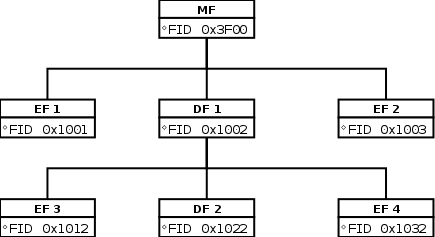
\includegraphics[width=0.7\textwidth]{image/fs_example.png}
\caption{struktur file system}
\label{fig-fs-example}
\end{figure}

\subsubsection{Atribut File}
\label{file-attribute}

Setiap file pada \textsl{smart card} dikenali melalui FID dari file tersebut. Untuk mencegah ambiguitas, maka file-file yang berada dalam 1 DF tidak boleh memiliki FID yang sama (demikian pula dengan DF induknya). 

Dilihat dari sisi penggunanya, \emph{Elementary File} (EF) dibagi menjadi dua jenis, yaitu :
\begin{itemize}
\item Working EF, dan 
\item Internal EF.
\end{itemize}

 \emph{Working} EF adalah EF yang menyimpan data-data milik aplikasi \textsl{smart card} dan dapat diakses oleh aplikasi. Sementara \emph{internal} EF adalah EF yang menyimpan data-data milik \emph{operating system} dan tidak dapat diakses langsung oleh aplikasi. Contoh \emph{internal} EF misalnya adalah file EF yang menyimpan kunci keamanan. Kunci yang disimpan dalam file ini akan dibaca oleh \emph{operating syste}m dan dicocokkan dengan kunci yang diberikan oleh pengguna \textsl{smart card} untuk memperoleh hak untuk mengakses file-file lainnya didalam DF.

Standar ISO 7816-4 memberikan 5 struktur internal berbeda yang mungkin digunakan pada sebuah file EF, yaitu :
\begin {itemize}
\item Transparent
\item Linier Record (fixed length)
\item Linier Record (variable length)
\item Cyclic Record
\item TLV
\end {itemize}

Selain jenis (\emph{working} atau \emph{internal}) dan struktur internalnya EF, terdapat sejumlah atribut lainnya yang dapat melekat pada sebuah file, diantaranya :
\begin {itemize}
\item read-write/read-only
\item shareable/not-shareable
\item access condition
\end {itemize}

\subsubsection{Operasi file}
\label{file-operation}

Sebagaimana pada sistem komputer lainnya, pengguna dapat melakukan sejumlah operasi terhadap file. Operasi-operasi file yang dapat dilakukan pada \textsl{smart card} mencakup:

\begin{itemize}
\item Menciptakan file
\item Menghapus file
\item Memilih file
\item Menulis file
\item Membaca file
\item Mengubah atribut file
\end{itemize}

\subsubsection{Keamanan file}
\label{file-security}

Salah satu faktor penting yang menjadi kelebihan \textsl{smart card} dibanding kartu elektronik lainnya adalah dari segi keamanan. Demikian pula terhadap file yang disimpan didalamnya (dalam hal ini oleh \emph{file system}). Untuk mencapai tingkat keamanan tersebut, pengguna harus terlebih dahulu memenuhi kondisi tertentu untuk dapat mengakses sebuah file. Kondisi yang diperlukan ini selanjutnya disebut juga sebagai \emph{Access Condition} (AC). Metode yang akan digunakan untuk mengimplementasikan \emph{access condition} ini adalah dengan menggunakan \emph{security state}. Pada metode ini, pengguna harus mencapai \emph{security state} tertentu (melalui verifikasi PIN) untuk dapat mengakses sebuah file. \emph{Security state} yang dibutuhkan dapat berbeda untuk setiap operasi, sehingga dibutuhkan sebuah access condition untuk setiap operasi. 

\begin{itemize}
\item access condition untuk membaca,
\item access condition untuk menulis,
\item access condition untuk menghapus file,
\item access condition untuk menciptakan file baru (khusus DF).
\item access condition untuk mengubah atribut
\end{itemize}
